\chapter{VALIDAÇÃO DOS MODELOS}
\label{validacao}
\section{\textbf{Introdução}}
Neste capítulo serão apresentadas as validações realizadas com x exemplos conhecidos amplamente na literatura.
As validações são comparações entre os resultados numéricos obtidos pela modelagem apresentada e resultados gerados por soluções analíticas conhecidas. Elas foram separadas em três grupos que representam diferentes tipos de etapas do cálculo, desse forma espera-se demonstrar a qualidade do modelo em todas as etapas e relacionar o histórico de aprendizado e desenvolvimento do código.
São utilizadas as soluções analíticas unidimensionais dos problemas para que se possa comparar os resultados pois estas são as soluções presentes na literatura. Como os resultados são obtidos para problemas bidimensionais é preciso fazer a comparação entre resultados tomando uma seção da solução como referência, usualmente perto do meio. Essa adaptação dos dados gera uma aproximação dos resultados.

O primeiro grupo são os problemas em sólidos, que buscam confirmar a construção correta das matrizes de elementos, a aplicação apropriada dos diferentes tipos de condições de contorno e a solução de um modelo mais simples.
O segundo grupo trata dos exemplos de problemas com fluidos. 
Nesta etapa verifica-se novamente a construção das matrizes e aplicação das condições de contorno, 
porém o foco principal destes exemplos é validar o modelo e analisar as restrições de aplicabilidade.
Para o terceiro e último grupo de validações são trabalhados problemas clássicos em partículas.
São realidados testes para validar cada força trabalhando isoladamente, dessa forma facilita-se a correção pontual no modelo e pode-se comprovar com maior certeza a influência correta das forças.

A execução do código e computação dos resultados foram realizados em um computador de uso pessoal com as seguintes especificações:
\begin{itemize}
    \item Dell Latitude E6410 com processador Intel® Core™ i5 CPU M 520 2.40GHz com 4 núcloes e 4Gb de memória RAM.
          O sistema operacional ubuntu 16.04 LTS e compilador Python 3.5.
\end{itemize}

\section{\textbf{Validações de Problemas em Sólidos}}

\subsection{\textbf{Equação de Laplace com Condições de Contorno de Dirichlet Permanente}}
O problema de troca de calor em uma placa é um dos exemplos clássicos utilizados para estudar as equações de transmissão de calor em sólidos. O mais simples destes é uma barra unidimensional sem geração de calor onde a temperatura é conhecida nas extremidades.
Como a malha do código foi desenvolvida para solução de problemas bidimensionais, cria-se um problema bidimensional com condições de contorno equivalentes e extrai-se uma seção para que se possa comparar os resultados.

A equação de governo é dada por:
\begin{equation}
    \nabla^2 T = 0
    \label{laplace_d_perm_eq} 
\end{equation}

O problema unidimensional é definido como:
\begin{itemize}
    \item $x\in [0,1]m$
    \item $T(0) = 0^{\circ}C$
    \item $T(1) = 1^{\circ}C$
\end{itemize}

As condições do problema bidimensional equivalente, ver \ref{laplace_d_perm_bc}, onde a seção tomada será em $x=0,5m$, é dado por:
\begin{itemize}
    \item $x,y\in [0,1]m$
    \item $T(0,y) = 0^{\circ}C$
    \item $T(1,y) = 1^{\circ}C$
    \item $\dfrac{dT}{dt}(x,0) = 0^{\circ}C/s$
    \item $\dfrac{dT}{dt}(x,1) = 0^{\circ}C/s$
\end{itemize}

\begin{figure}[!ht]
    \centering
    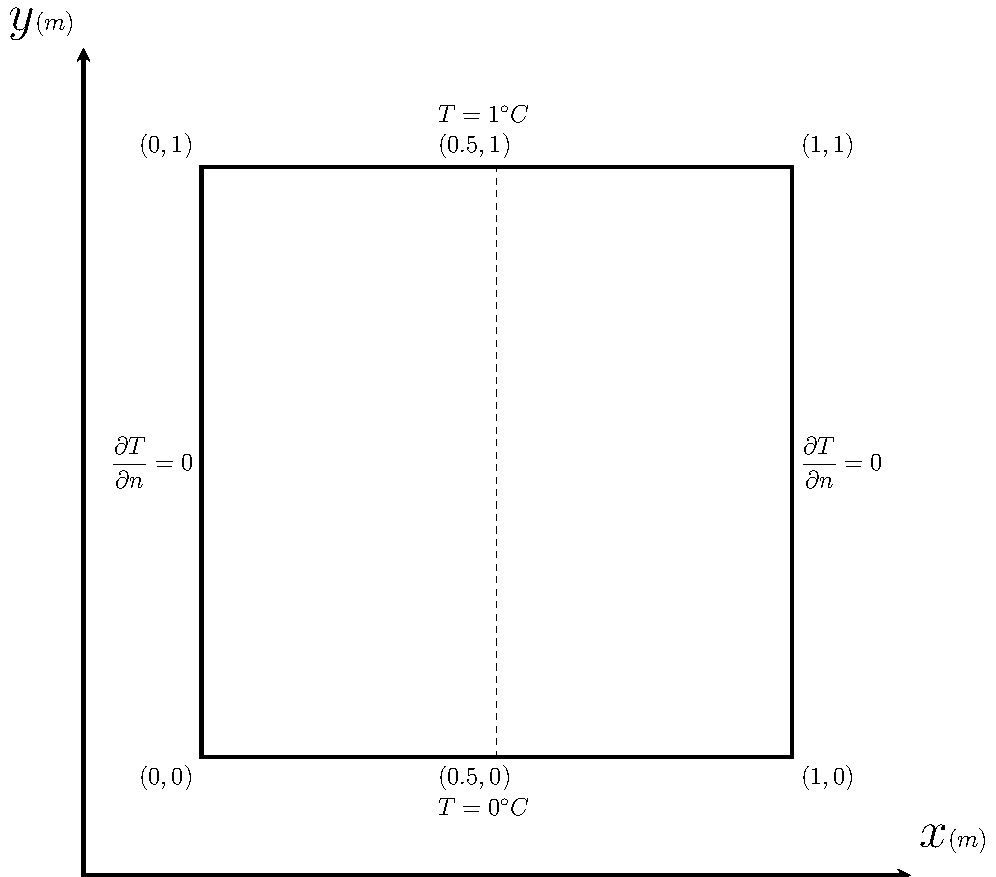
\includegraphics[width=.7\linewidth]{figures/laplace_dirichlet_boundary_conditions.pdf}
    \caption{Condições de contorno da placa.}
    \label{laplace_d_perm_bc}
\end{figure}

A solução analítica da equação \ref{laplace_d_perm_eq} deste problema é dada por:
\begin{equation}
    T(x) = C_1*x + C_0
    \label{laplace_d_perm_sol}
\end{equation}
Onde $C_0$ e $C_1$ são, respectivamente, as condições de contorno em $x=0m$ e $x=1m$.

A solução na placa bidimensional encontrada foi:
\begin{figure}[!ht]
    \centering
    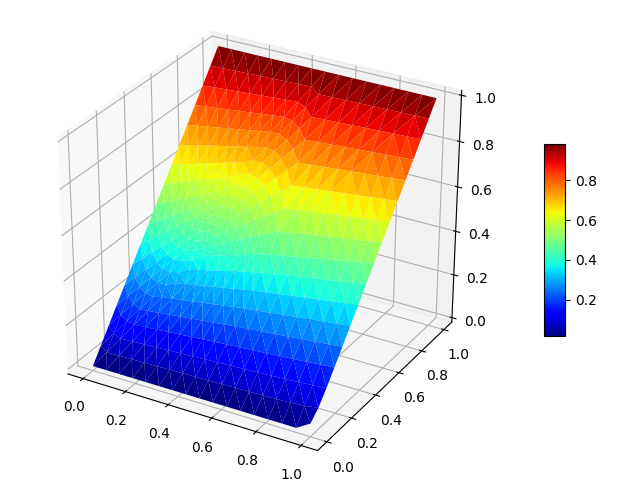
\includegraphics[width=.7\linewidth]{figures/laplace_dirichlet_permanent_3d.png}
    \caption{Distribuição de temperaturas na placa.}
    \label{laplace_d_perm_3d}
\end{figure}

